\documentclass[11pt]{article}
\usepackage[margin=1in]{geometry}
\usepackage{amsmath,amssymb}
\usepackage{url}
\usepackage{hyperref}
\usepackage{booktabs}
\usepackage{microtype}
\usepackage{tikz}
\usetikzlibrary{arrows.meta,positioning,fit,backgrounds,calc,patterns}

\newcommand{\package}[1]{\texttt{#1}}

\title{\package{QECCertificates}: checkable distance certificates\\
for quantum error correction}
\author{Shuoming An\\[4pt]
\small Faculty of Computility Microelectronics,\\
\small Shenzhen University of Advanced Technology, Shenzhen, Guangdong 518107,\\
\small China\\[3pt]
\small Guangdong Provincial Key Laboratory of Computility Microelectronics,\\
\small Shenzhen, Guangdong 518107, China\\[3pt]
\small Pengxin Quantum Technology (Shenzhen) Co., Ltd., Shenzhen 518107, China\\[3pt]
\small \texttt{anshuoming@suat-sz.edu.cn}}
\date{Draft of 30 September 2026}

\begin{document}
\maketitle

\begin{abstract}
A quantum computer fails unless the code that stores its information is good enough, and
one number measures how good that code is: the size of the smallest error it cannot
detect. Quantum low-density parity-check codes promise a favourable trade between that
number and the number of physical parts, and they are found by search, which enumerates
candidates and computes a distance for each. In practice the public data report such a
distance as an upper bound, because certifying it is expensive. A reader who wants to know
whether the number is real has to trust the program, or repeat the search. Here we show
that the check can be built from theorems instead of trust. The encoding that turns a code
into a satisfiability instance is faithful in both directions, so a model of the encoded
formula is exactly a light logical operator, and the checker that reads a solver's
refutation is sound. A distance claim can then be closed by a kernel that never saw the
search. The
closest previous route replays the solver's proof inside a proof assistant, and its
authors report that at 144 qubits the replay is the wall; separating search from check
keeps the expensive part outside the trusted base. Fifty-seven Lean~4 modules carry the
algebra, the translation from Pauli operators to bit-vectors and the code instances, and
every non-private theorem and lemma is printed in an audit region whose statements rest on
the three axioms the kernel's logic needs. A certificate that is checkable without the
tool that produced it can travel to other constructions and other solvers, and two
companion developments already import the library as the home of their shared statements.
\end{abstract}

\section{Why this exists}

Quantum low-density parity-check codes are designed by search: choose a construction,
enumerate candidates, compute a distance. The public schema behind the qLDPC
Challenge~\cite{qldpc} records what a search leaves open. A distance that is not certified
is reported there as an upper bound, for a non-CSS code because the Pauli-weight
certifier ``is not available yet'' and for a circuit-level distance because an exact tier
``is deferred future work''; what lies between an upper bound and a proof, the schema
calls evidence.\footnote{The quotations are from the schema's own descriptions of the
distance tiers, read on 30 September 2026. The wording is theirs, not ours.}

Two notions in that sentence name what is missing, and both need a word of explanation. A
CSS code is one whose parity checks split into two families, one measuring X-type errors
and one measuring Z-type; the Pauli-weight certifier is the component that would bound
how few qubits a logical operator touches. A circuit-level distance counts faults in the
syndrome extraction that reads those checks, not only faults in the stored codewords, and
its code-level analogue is what this paper calls a fault distance.

The nearest prior work on the kernel side, Lean-QEC~\cite{leanqec}, turns the distance
question into a satisfiability question and replays the solver's proof inside a proof
assistant. Its reported reach is 90 qubits, and its authors state that at 144 qubits the
replay itself is the wall.

This paper reports the library that supplies both halves of the check. A distance claim
becomes checkable when the search problem is encoded faithfully, so that solving the
encoded formula and finding a light logical operator are the same thing, and when the
refutation the solver returns is read by a checker whose soundness is a theorem. The
search may then be as fast, as heuristic and as untrusted as its users like, because it
is no longer part of the argument.

\begin{figure}[!htbp]
\centering
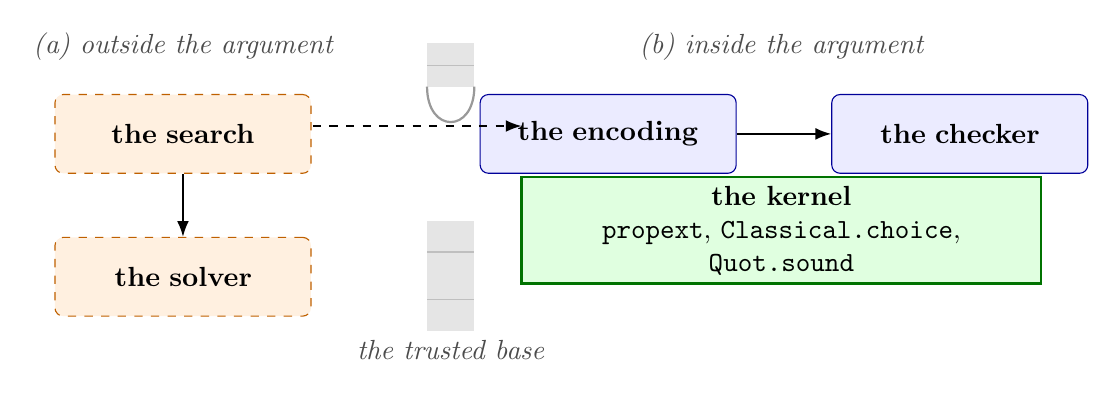
\begin{tikzpicture}[font=\normalsize,
  bx/.style={draw, rounded corners=3pt, align=center, inner sep=5pt,
             minimum height=1.0cm, text width=2.9cm},
  free/.style={bx, fill=orange!12, draw=orange!75!black, dashed},
  inb/.style={bx, fill=blue!8, draw=blue!60!black},
  krn/.style={bx, fill=green!10, draw=green!45!black},
  fl/.style={-{Latex[length=2mm]}, semithick},
  dfl/.style={-{Latex[length=2mm]}, semithick, dashed},
  panel/.style={font=\normalsize\itshape, text=black!70, inner sep=2pt}]

% (a) outside the argument
\node[free] (search) at (1.3,0.75) {\textbf{the search}};
\node[free, below=0.8cm of search] (solver) {\textbf{the solver}};
\draw[fl] (search) -- (solver);
\node[panel, anchor=south] at (1.3,1.6) {(a) outside the argument};

% (b) inside the argument, standing on the kernel
\node[inb] (enc) at (6.7,0.75) {\textbf{the encoding}};
\node[inb, right=1.2cm of enc] (chk) {\textbf{the checker}};
\draw[fl] (enc) -- (chk);
\node[panel, anchor=south] at (8.9,1.6) {(b) inside the argument};
\fill[green!12] (5.6,0.2) rectangle (12.2,-1.15);
\draw[green!45!black, thick] (5.6,0.2) rectangle (12.2,-1.15);
\node[align=center] at (8.9,-0.48)
  {\textbf{the kernel}\\ \texttt{propext}, \texttt{Classical.choice},\\ \texttt{Quot.sound}};

% the wall, with an archway that the one crossing object passes through
\fill[black!10] (4.4,1.9) rectangle (5.0,1.35);
\fill[black!10] (4.4,-0.35) rectangle (5.0,-1.75);
\foreach \y in {1.62,-0.75,-1.35}{\draw[black!25] (4.4,\y) -- (5.0,\y);}
\draw[black!40, thick] (4.4,1.35) .. controls (4.4,0.75) and (5.0,0.75) .. (5.0,1.35);
\node[panel, anchor=north] at (4.7,-1.8) {the trusted base};
\draw[dfl] (2.95,0.85) -- (5.6,0.85);
\end{tikzpicture}
\caption{A distance claim crosses the wall as one object: the claim itself, and the file of
steps that is supposed to certify it. The search and the solver may be as heuristic as they
like, because everything beyond the wall is checked, and both rooms stand on the kernel.}
\label{fig:trusted-base}
\end{figure}

\section{What is in the library}

\package{QECCertificates} is a Lean~4 development of 57 modules on Lean 4.34, built
against mathlib at a pinned revision, on the same toolchain as the two developments that
consume it.

\begin{itemize}
\item \textbf{A layer for the two-element field.} Vectors over that field, row spaces, a trusted
row reduction with a proved pivot invariant, kernel bases, membership decisions that are
computable, weight-limited enumeration with a covering theorem, and a certificate for a
distance lower bound as a single decidable predicate.
\item \textbf{An operator layer.} Pauli expressions with a symplectic representation, in
which a Pauli operator is recorded by two bit-vectors per qubit saying whether it carries
an X and whether it carries a Z, and translation theorems that make the vector-level
decisions equal to statements about the matrices the surrounding ecosystem uses.
\item \textbf{A certificate framework.} An in-kernel checker for LRAT proofs, the format
in which a satisfiability solver records its refutation~\cite{cade2017}, with a proof that
the checker is sound; a formalization of the encoding step that ties satisfiability of the
encoded formula to the existence of a light logical operator, in both directions; and
symmetry breaking by lex-leader predicates, which keep the lexicographically smallest
representative of each symmetry orbit, with the faithfulness of the reduction proved
rather than assumed.
\item \textbf{Instances.} Kernel-checked assertions of the triple $(n,k,d)$, the number
of physical qubits, of logical qubits and the least weight of an undetected logical error,
for a table of codes, including a hypergraph-product family covered by general theorems
rather than by instance-by-instance evaluation.
\end{itemize}

\section{What is checked, and how}

Two properties are meant to be machine-checked rather than asserted, because both are the
kind of claim that is either checked or is marketing. What a claim becomes is worth
stating once, because the two shapes of a certified bound are not symmetric: the lower
bound has to exclude every light operator and needs a solver for it, while the upper bound
is one operator away.

\begin{figure}[!htbp]
\centering
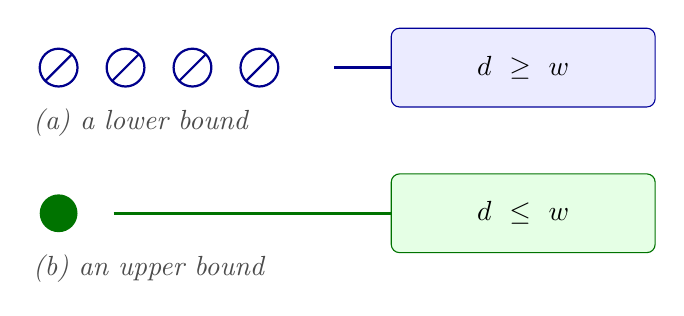
\begin{tikzpicture}[font=\normalsize,
  bx/.style={draw, rounded corners=3pt, align=center, inner sep=5pt,
             minimum height=1.0cm, text width=3.0cm},
  inb/.style={bx, fill=blue!8, draw=blue!60!black},
  wit/.style={bx, fill=green!10, draw=green!45!black},
  fl/.style={-{Latex[length=2mm]}, semithick},
  panel/.style={font=\normalsize\itshape, text=black!70, inner sep=2pt}]

% (a) a lower bound: every operator lighter than w has to be ruled out
\foreach \i in {0,1,2,3}{%
  \draw[blue!55!black, thick] (0.45+\i*0.85,0) circle (0.24);
  \draw[blue!55!black, thick] (0.28+\i*0.85,-0.17) -- (0.62+\i*0.85,0.17);}
\draw[->, very thick, blue!55!black] (3.95,0) -- (5.1,0);
\node[inb] (lb) at (6.35,0) {\textbf{$d \ge w$}};
\node[panel, anchor=north west] at (0.05,-0.45) {(a) a lower bound};

% (b) an upper bound: one operator at the weight w is enough
\fill[green!45!black] (0.45,-1.85) circle (0.24);
\draw[->, very thick, green!45!black] (1.15,-1.85) -- (5.1,-1.85);
\node[wit] (ub) at (6.35,-1.85) {\textbf{$d \le w$}};
\node[panel, anchor=north west] at (0.05,-2.3) {(b) an upper bound};
\end{tikzpicture}
\caption{The two shapes of a certified bound, and why they are not symmetric. A lower
bound in panel (a) has to rule out every logical operator lighter than the claimed weight
$w$, which is why it needs a search and a solver. An upper bound in panel (b) is a single
operator of weight $w$: write one down, have its weight checked, and the distance is at
most $w$. The library spends its machinery on the left-hand side.}
\label{fig:two-bounds}
\end{figure}

\paragraph{The trusted base.} No declaration in the library uses \package{sorry}, a custom
axiom, or \package{native\_decide}; the computations that matter are carried out by the
kernel itself, so a proof that leans on such a computation is a proof the kernel has
already performed. The root module carries an audit region of 1{,}071 lines, each a
request that the kernel print the axioms one load-bearing declaration depends on, and the
region covers every non-private theorem and lemma in the package. A script in
\package{tools/} reads those lines out of a build log and fails on any axiom outside
\package{propext}, \package{Classical.choice} and \package{Quot.sound}; it fails as well
when the log carries no output at all, so a clone that was never built is not a pass.

\paragraph{The build.} Continuous integration builds the library on a hosted runner, and
holds the result to zero error lines and zero warnings from this package's own files. Not
all of it fits. Eleven modules close their statements by kernel reduction over an object
large enough to need tens of gigabytes, and the largest of them needs 77 GiB, so the job
builds the 25 modules whose measured peak fits a runner, together with everything those
modules import. A table in the repository records the peak of every module and fails the
build when the tree and the table disagree, so a new module is measured before it is built
anywhere. The audit region is the root module, which imports the whole library, so the
audit runs on a machine where the full build fits, and each run says in its log what it
left out.

\section{How the two companion developments use it}

The library is the shared core of two further developments. One builds an interface layer
in which the row space defined here is proved equal to the row space of Lean-QEC, the
symplectic predicate is proved equivalent to commutation of actual Pauli matrices, and a
state on the logical register is bounded by the logical dimension proved here. The other
builds fault complexes, the gauge-fixed instances, and a layer of conditions under which a
logical measurement succeeds, all on the same core. Both pin the package by commit, and
the papers that report those results cite this library as the home of the shared
statements, so a reader can check the interface claims without reading either paper's
repository.

\section{Using it}

\begin{verbatim}
    # in a lakefile.toml
    [[require]]
    name = "QECCertificates"
    git = "https://github.com/QCL-SUAT/QECCertificates.git"
    rev = "<40-hex commit>"

    lake exe cache get   # prebuilt mathlib, on a machine that has not built it
    lake build
\end{verbatim}

Nothing is configured per machine: every dependency is fetched at a pinned revision, and
a script that links a local prebuilt layer is optional and never required for a build to
succeed. The released version is archived at
\url{https://doi.org/10.5281/zenodo.23056679}, which is what to cite. The audit region is
part of the build, so a downstream user sees the axiom list for the statements they
consume in their own build log.

\section{What it does not do}

The library does not simulate circuits, decode syndromes, or enumerate codes; those are
served by mature projects, and the point of a certificate layer is to sit beside them
rather than to reimplement them. It does not claim a general decision procedure for
distances: what it offers is a format in which a bound, once found, is checkable, and a
kernel that decides the check. It does not accept a solver's word at any step: the
in-kernel path closes the argument with a proof object, and the certificate toolchain that
lands next is written so that the checker is independent of the solver that produced the
proof. Finally, it does not carry the code tables of the field: a handful of instances are
included because they are load-bearing for the two companion developments, not as a
database.

\section{Conclusion}

A distance claim can now be checked without repeating the search. The library supplies a
proof object a third party can check, an audit region that prints the axioms behind every
statement, and a checker that shares no code with the solver. The Python certificate chain
follows: the CNF encoder for distance lower bounds with a known-value gate, LRAT and RUP
checkers written twice in different languages so that a bug in one is unlikely to be
mirrored in the other, and the adapters that turn a check matrix into a certified bound. A
later white paper will report that chain's end-to-end results on the instances the two
companion developments use.

\begin{thebibliography}{9}
\bibitem{leanqec} M.~Ehatamm, Y.~Lee, X.~Wu and R.~Tao, \emph{End-to-End
Formalization of Quantum Error Correction}, arXiv:2605.16523 (2026).
\bibitem{cade2017} L.~Cruz-Filipe, M.~J.~H.~Heule, W.~A.~Hunt, M.~Kaufmann and
P.~Schneider-Kamp, \emph{Efficient certified RAT verification}, in Automated
Deduction (CADE-26), LNCS 10395, 220--236 (2017).
\bibitem{qldpc} The qLDPC Challenge, public data schema and tier descriptions,
\url{https://github.com/unitaryfoundation/qldpc-challenge} (read 30 September 2026).
\end{thebibliography}

\end{document}
